\documentclass[12pt]{beamer}
\setbeamertemplate{navigation symbols}{}%remove navigation symbols
\usepackage{booktabs}
\usepackage{multicol}
\usepackage{transparent}
\usepackage{soul}
\usepackage{ulem}
\usepackage{wasysym}
\usepackage{hyperref}
\usepackage{subcaption}
\usepackage{listings}
\usepackage{fancyvrb}
\usepackage{multicol}
\usepackage{booktabs}
\usepackage[document]{ragged2e}
\usepackage[english]{babel}
\usepackage{blindtext}
\usepackage{ragged2e}
\usepackage{adjustbox}
\usepackage{amsmath}
\usepackage{tcolorbox}
\usepackage{graphicx}
\usepackage{animate}
\renewcommand{\ULthickness}{1pt}
\captionsetup{justification=raggedright,singlelinecheck=false}

\newenvironment{myenv}[1]
  {\mdfsetup{
    frametitle={\colorbox{white}{\space#1\space}},
    innertopmargin=0pt,
    frametitleaboveskip=-\ht\strutbox,
    frametitlealignment=\center,
    linewidth=1pt,
    roundcorner=10pt
    }
  \begin{mdframed}%
  }
  {\end{mdframed}}

\useoutertheme{infolines}
\usepackage{newpxtext,newpxmath}
%\usepackage{mathpazo}

\usepackage[framemethod=tikz]{mdframed}
\usetikzlibrary{shadows}
\usepackage{pdfpages}
\newmdenv[shadow=true,shadowcolor=black,font=\sffamily,rightmargin=8pt]{shadedbox}
\usepackage{pifont,xcolor}
\definecolor{myblue}{RGB}{49,54,149}
\definecolor{myred}{RGB}{165,0,38}

\definecolor{myorange}{RGB}{255,120,0}
\definecolor{mygreen}{RGB}{76, 187, 23}

\definecolor{grayedout}{RGB}{225,225,225}
\usepackage{graphicx}
\usepackage{caption}
\usepackage{amsmath}
\newcommand{\icol}[1]{% inline column vector
  \left(\begin{smallmatrix}#1\end{smallmatrix}\right)%
}
\newcommand{\lenitem}[2][.55\linewidth]{figures//\parbox[t]{#1}{#2\strut \strut \justify \justifying}}

\usetheme{Frankfurt}

%   \usefonttheme{professionalfonts}
\newenvironment{variableblock}[3]{%
  \setbeamercolor{block body}{#2}
  \setbeamercolor{block title}{#3}
  \begin{block}{#1}}{\end{block}}
\usecolortheme{dove}
%\usecolortheme{rose}
%\usecolortheme{whale}

\usefonttheme[onlymath]{serif}  % only math serif font
\usefonttheme{serif}

\setbeamercolor{block title}{bg=white,fg=black}
\newcommand{\itemcolor}[1]{% Update list item colour
  \renewcommand{\makelabel}[1]{\color{#1}\hfil ##1}}

\newcounter{tmpc}
\setbeamercolor{section in head/foot}{fg=black, bg=white}
\setbeamercolor{enumerate item}{ fg=myred}
\setbeamertemplate{frametitle}
{
    \nointerlineskip
    \begin{beamercolorbox}[sep=0.3cm,ht=1.8em,wd=\paperwidth]{frametitle}
        \vbox{}\vskip-3ex%
        \strut\insertframetitle\strut
        \vskip-1.2ex%
    \end{beamercolorbox}
}
\addtobeamertemplate{frametitle}{\vskip0.5ex}{}
\makeatletter
\setbeamertemplate{footline}
{
  \leavevmode%
  \hbox{%
  \begin{beamercolorbox}[wd=.875 \paperwidth,ht=2.25ex,dp=1ex,left]{section in head/foot}%
    \usebeamerfont{author in head/foot}\quad \quad \insertshorttitle
 \end{beamercolorbox}%
 \begin{beamercolorbox}[wd=.125\paperwidth,ht=2.25ex,dp=1ex,right]{section in head/foot}%
    \usebeamerfont{date in head/foot} \quad \quad
    \insertframenumber{} / \inserttotalframenumber\hspace*{2ex}
  \end{beamercolorbox}}%
  \vskip0pt%
}
\let\@@magyar@captionfix\relax



\newcommand\jsonkey{\color{purple}}
\newcommand\jsonvalue{\color{cyan}}
\newcommand\jsonnumber{\color{orange}}

% switch used as state variable
\makeatletter
\newif\ifisvalue@json

\lstdefinelanguage{json}{
    tabsize             = 4,
    showstringspaces    = false,
    keywords            = {false,true},
    alsoletter          = 0123456789.,
    morestring          = [s]{"}{"},
    stringstyle         = \jsonkey\ifisvalue@json\jsonvalue\fi,
    MoreSelectCharTable = \lst@DefSaveDef{`:}\colon@json{\enterMode@json},
    MoreSelectCharTable = \lst@DefSaveDef{`,}\comma@json{\exitMode@json{\comma@json}},
    MoreSelectCharTable = \lst@DefSaveDef{`\{}\bracket@json{\exitMode@json{\bracket@json}},
    basicstyle          = \ttfamily
}

% enter "value" mode after encountering a colon
\newcommand\enterMode@json{%
    \colon@json%
    \ifnum\lst@mode=\lst@Pmode%
        \global\isvalue@jsontrue%
    \fi
}

% leave "value" mode: either we hit a comma, or the value is a nested object
\newcommand\exitMode@json[1]{#1\global\isvalue@jsonfalse}

\lst@AddToHook{Output}{%
    \ifisvalue@json%
        \ifnum\lst@mode=\lst@Pmode%
            \def\lst@thestyle{\jsonnumber}%
        \fi
    \fi
    %override by keyword style if a keyword is detected!
    \lsthk@DetectKeywords%
}


\makeatother

\def\mf{
\begin{itemize}
\item Item
\end{itemize}
}
\setbeamercolor{item projected}{bg=myblue}
\setbeamertemplate{enumerate items}[default]
\setbeamertemplate{navigation symbols}{}
%\setbeamercovered{transparent}
\setbeamercolor{block title}{fg=myred}
\setbeamercolor{local structure}{fg=myred}

\usepackage{listings}

\lstdefinestyle{BashInputStyle}{
  language=bash,
  basicstyle=\small\sffamily,
  numbers=left,
  numberstyle=\tiny,
  numbersep=5pt,
  framexleftmargin=3mm,
  frame=shadowbox, rulesepcolor=\color{gray},
  numberstyle=\normalfont\tiny\color{myred},
  rulecolor=\color{black},
  columns=fullflexible,
  backgroundcolor=\color{white},
  linewidth=0.9\linewidth,
  xleftmargin=0.1\linewidth
}

\begin{document}

\section{Introduction and Motivation}
\setstcolor{red}

\title{On the Responsible use of Pseudo-Random Number Generators in Scientific Research} \vspace{-0.25in}
\author{\footnotesize{Charlie Rahal\\ \vspace{0.05in} LCDS and Nuffield College, University of Oxford\\\vspace{.1in}Xi'an Jiaotong, 2024}\\ \vspace{-0.15in}}
 \date{}
\frame{\titlepage
\begin{center}
\vspace{-.6in}
\begin{figure}
\centering
\begin{subfigure}{.5\textwidth}
  \centering
  \includegraphics[width=.55\linewidth]{figures/LCDS_Logo_SVG_BlackOrange.pdf}
\end{subfigure}%\hspace{-.05in}
\hspace{.01in}\begin{subfigure}{.45\textwidth}
  \centering
  \includegraphics[width=.45\linewidth]{figures//Uni_Oxford_logo.pdf}
\end{subfigure}
\end{figure}
 \end{center}
}

\begin{frame}
\frametitle{What is a PRNG?}
\begin{figure}
	\includegraphics[width=0.95\textwidth]{figures/chat_gpt.png}
\end{figure}
\end{frame}

\begin{frame}
\frametitle{Pseudo-Random Number Generation}
An invisible source of uncertainty in the scientific record: PRNGs! \\ \vspace{.05in} \pause
	\begin{itemize}
		\item \textbf{Q}: Has anyone ran a program twice, with different results?\\ \vspace{.1in}\pause
		\item \textbf{Q}: Has anyone here ever set a `\color{myblue}seed\color{black}'? Which seed?\\ \vspace{.1in}\pause
		\item Maybe to eliminate variation in algorithms with PRNGs?\\ \vspace{.05in}
		\begin{itemize}
		\item[-] This seems to be the current `best practice' advice.\\ \vspace{.1in}  \pause
		\end{itemize}
			\item We argue this is the \color{myred}opposite of what we want\color{black}!\\ \vspace{.05in}
			\begin{itemize}
				\item[-] We propose you pre-specify \textbf{multiple} (complex) seeds.\\ \vspace{.05in} \pause
				\item[-] Or, alternatively, use a subset of the seeds \textbf{we} provide.
			\end{itemize}
	\end{itemize}
\end{frame}

\begin{frame}
\frametitle{Pseudo-Random Number Generation (Cont.)}
	\begin{itemize}
 		\item We \sout{want} need to assess possible variation independent of arbitrary seed choice.\vspace{.1in}\pause
		\item An extremely important and scarcely researched problem.\vspace{.1in}\pause
		\item Pseudo-Random Number Generators occur \color{myblue}everywhere\color{black}!\\ \vspace{.1in}\pause
		\item The variation in estimand can be \color{myblue} \textbf{huge} \color{black} (as we'll show).\\ \vspace{.1in}\pause
		\item We bring attention to this through multiple types of replications.\\ \vspace{.05in}
		\begin{itemize}
			\item Simulations, machine learning, NLP, and inferential research.\\ \vspace{.05in}
		\end{itemize}
		\item Seed variation at times: i.) can be eliminated, ii.) is not a concern, iii.) cannot be eliminated (requires examination).
	\end{itemize}
\end{frame}


\begin{frame}
\frametitle{The General Premise}
\begin{itemize}
\item \textbf{\color{myred}Problem Statement\color{black}}: By setting \textbf{one} seed, we ignore the variation of our estimand as a function of how PRNGs were generated: computationally un-intensive, but scientifically dour.\\ \pause \vspace{.2in}
\item \textbf{\color{myred}Solution\color{black}}: Visualize the outcome space of a \textbf{large number} (10k? 100k?) of seeds simultaneously. This is computationally intensive, but scientifically faithful.\\ \pause \vspace{.2in}
\item \textbf{\color{myred}Replication\color{black}}: Similar to specification curves and p-hacking, we can consider whether an original result is in the tail/IQR of the distribution of possible outcome space.
\end{itemize}
\end{frame}


\section{Simple Simulations}
\begin{frame}
\begin{center}
\begin{figure}
	\includegraphics[width=0.85\textwidth]{../../figures/four_simple_examples.pdf}
\end{figure}
\end{center}
\end{frame}

\section{More Complex Replicaitons}
\begin{frame}
\begin{center}
\begin{figure}
	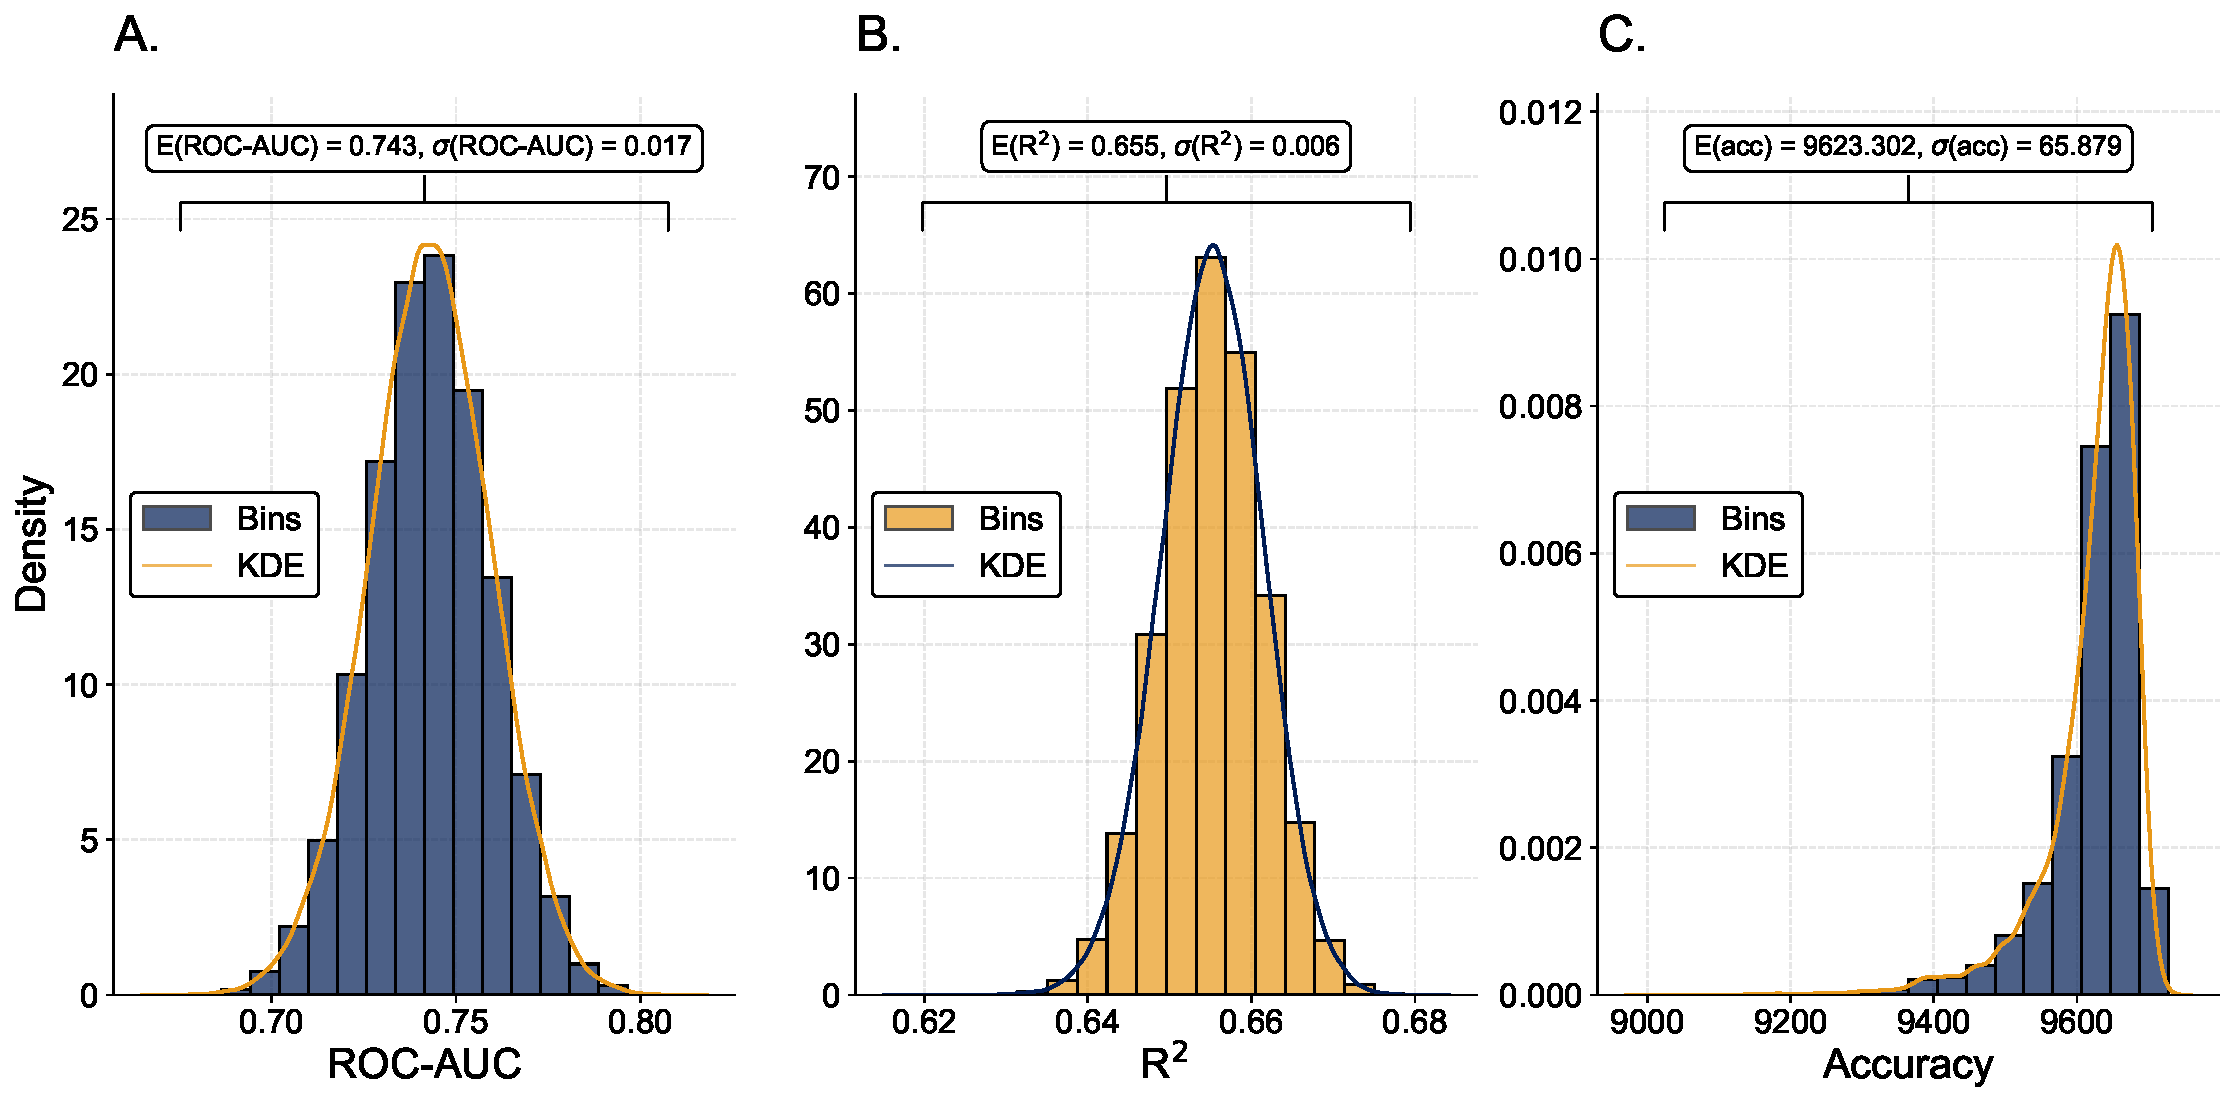
\includegraphics[width=\textwidth]{../../figures/prediction_seeds.pdf}
\end{figure}
\end{center}
\end{frame}

\begin{frame}
\begin{center}
\begin{figure}
	\includegraphics[width=0.95\textwidth]{../../figures/topic_modelling_seeds_histplot.pdf}
\end{figure}
\end{center}
\end{frame}

\begin{frame}
\begin{center}
\begin{figure}
	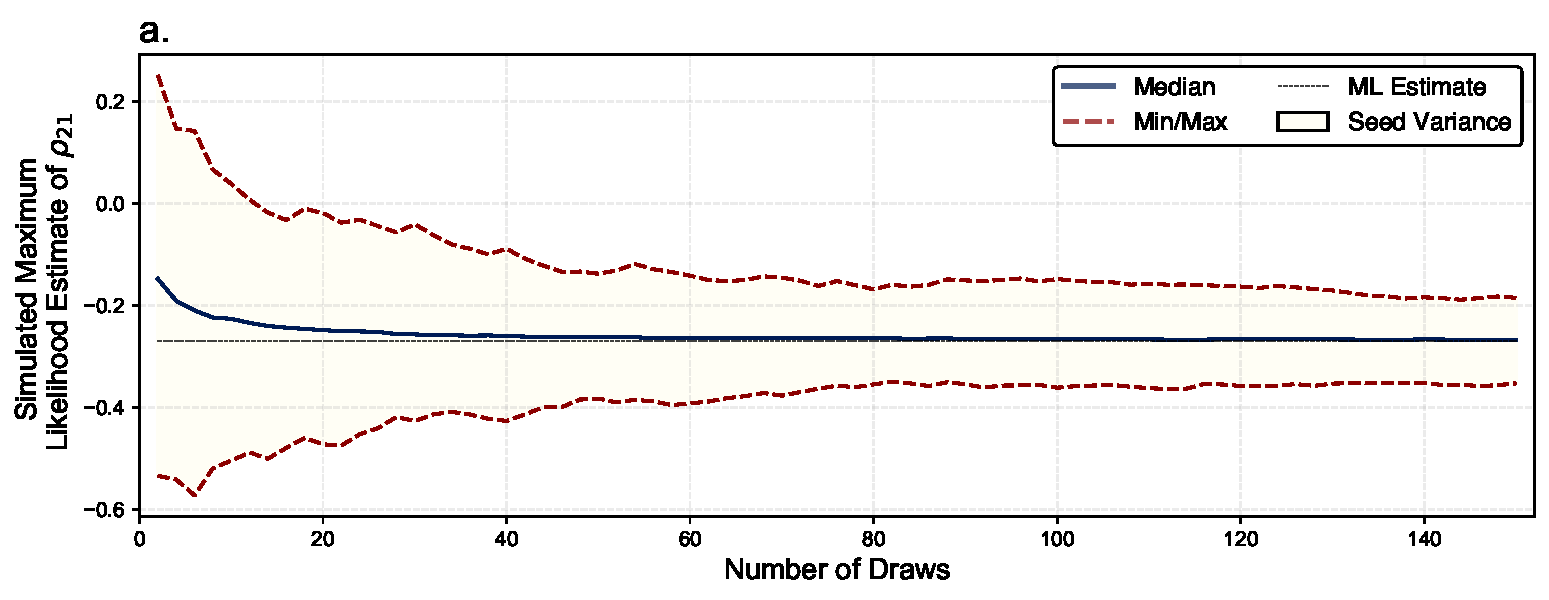
\includegraphics[width=0.95\textwidth]{../../figures/mvprobit.pdf}
\end{figure}
\end{center}
\end{frame}

\begin{frame}
\begin{center}
\begin{figure}
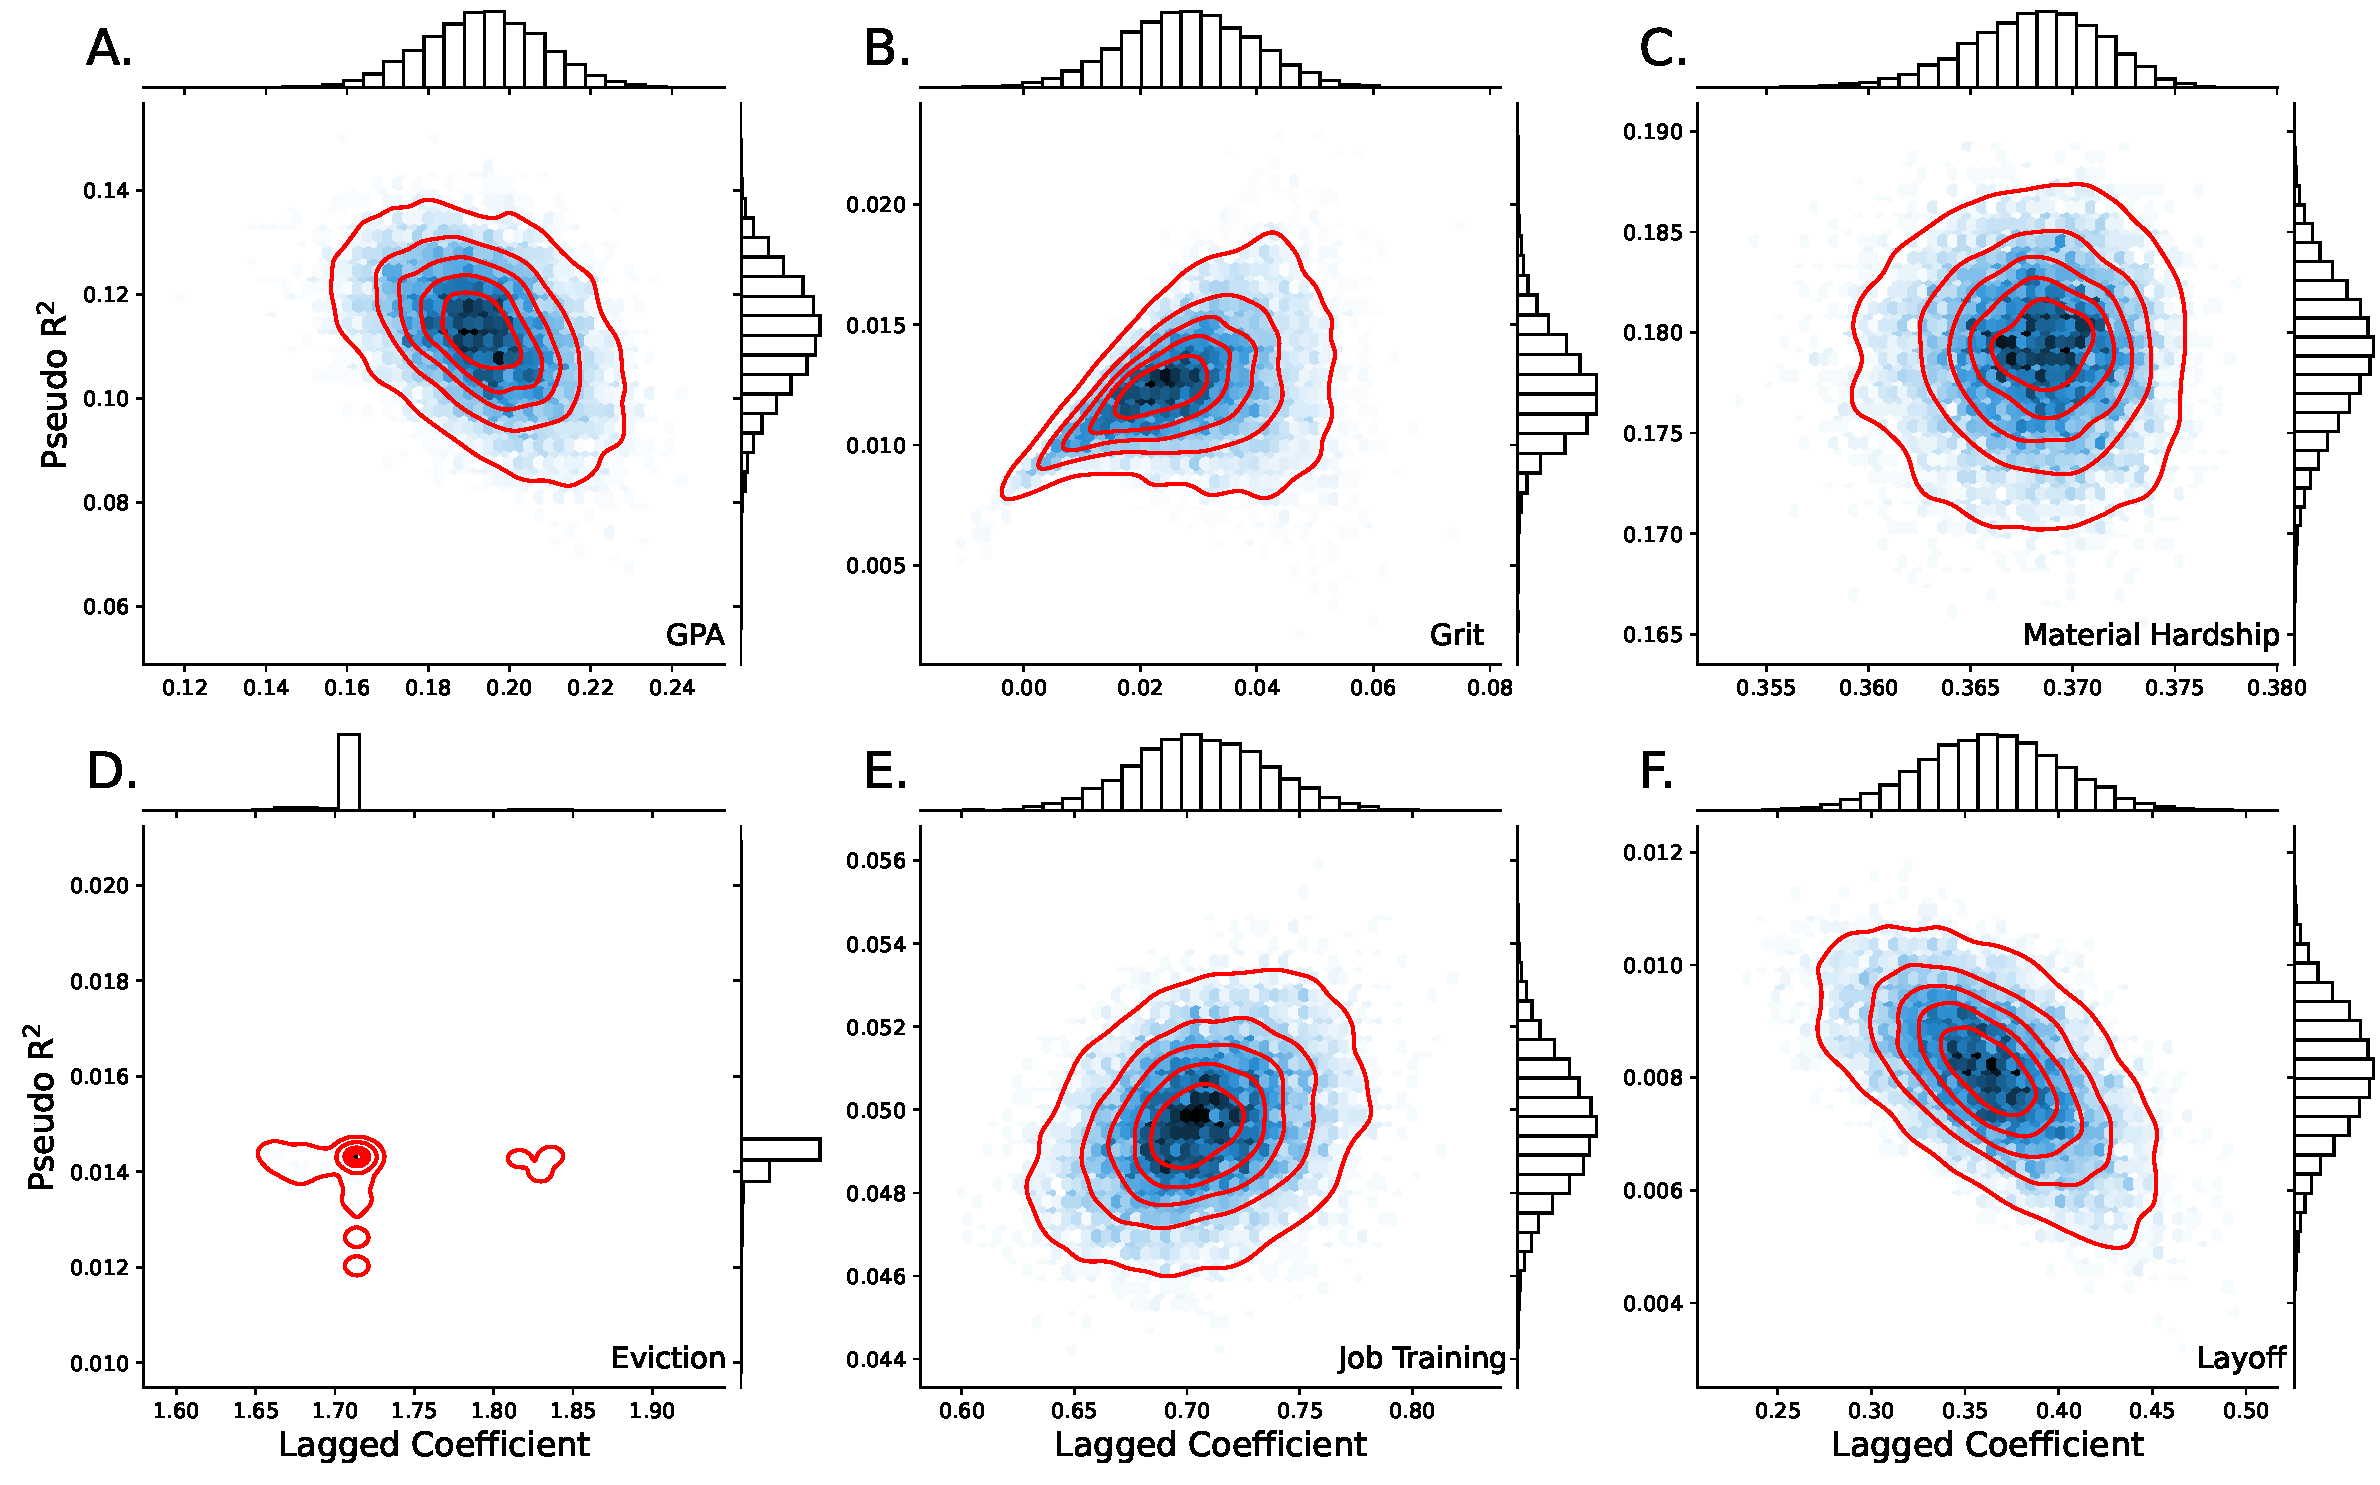
\includegraphics[width=.925\linewidth]{../../figures//ffc_seeds.pdf} \\ \vspace{.025in}
\end{figure}
\end{center}
\end{frame}

%\section{Collisions}
%\begin{frame}
%\begin{small}
%\frametitle{To make things more complicated...}
%\begin{itemize}
%\item Hofert (2020): in \textit{some} scenarios, \textbf{collisions} exist.\\ \vspace{.01in}
%\item Collisions: generation of duplicates b/c of insufficient complexity.\\ \vspace{.01in}
%\item An author of a leading LCDS publication recently  stated to me:\\ \vspace{.01in}
%\end{itemize}
%\begin{quote}
%\begin{small}
%\begin{center}
%``We wanted to run it [the model] with a 100k seeds, but in reality, it was only 99,905 or something, %because we were seeing that our results weren't unique when they should have been.''
%\end{center}
%\end{small}
%\end{quote}
%\begin{itemize}
%\item This \textit{only} occurs in 32-bit Mersenne Twister implementations.\\ \vspace{.01in}
%\begin{itemize}
%\item With 32-bit MT: E(collisions) is 116.\\ \vspace{.01in}
%\item With 64-bit MT: E(collisions is 2.71e-08.\\ \vspace{.01in}
%\end{itemize}
%\item The default implementation of MT in \texttt{R} is 32-bit$\hdots$.
%\end{itemize}
%\end{small}
%\end{frame}

%\begin{frame}
%\begin{center}
%\begin{figure}
%\includegraphics[width=.925\linewidth]{../../figures//collisions} \\ \vspace{.025in}
%\end{figure}
%\end{center}
%\end{frame}


\section{Concluding Thoughts}
\begin{frame}
\frametitle{Concluding Thoughts}
\begin{itemize}
\item Matt Salganik commented: `That sounds great, but expensive!'\\ \vspace{.1in}
\begin{itemize}
\item Expense no-longer prohibitive: everything here ran locally.\\ \vspace{.1in}
\end{itemize}
\item Does anyone have ideas for other types of seed variability?\\ \vspace{.1in}

\item Can this be corrective? Index historical seed variability?\\ \vspace{.1in}

\item Prospectively: we make available a list of seeds (replication materials), encouraging their use as a pre-specified set.\\ \vspace{.1in}

\item \textbf{TLDR}: when variation can't be eliminated, should be visualised.


\end{itemize}
\end{frame}

\end{document}
